\chapter{\label{method}Data Analysis}
The data analysis was performed using Python's \texttt{SciPy} library. We recorded the data for 20 combinations of masses attached to the oscillators and then for each file, the fitted parameters were found. Corresponding to each fit parameter, we found the the Rabi model parameters of $ Delta $ (detuning) and $ \Omega $ (Rabi frequency). Then these parameters of the Rabi model were themselves fit according to their equations, relating them with geometric phase.

For error analysis, we used Python's  \texttt{uncertainties} package, which preserved the significant digits when propagating errors. The complete code is on my \href{https://github.com/peakcipher/p442-integrated-lab/tree/master/IV.%20Coupled%20Oscillator}{GitHub}. Some snippets are also attached with this report.

In this section, we present our plots. In figure \ref{fig:first}, we present the fitted curve for one of the data file (representing one mass combination for the coupled oscillator). The figure \ref{fig:first_sq} represents the squares of the normalised amplitudes (basically the peaks of the `carrier' wave).

\begin{figure}[H]
	\centering
	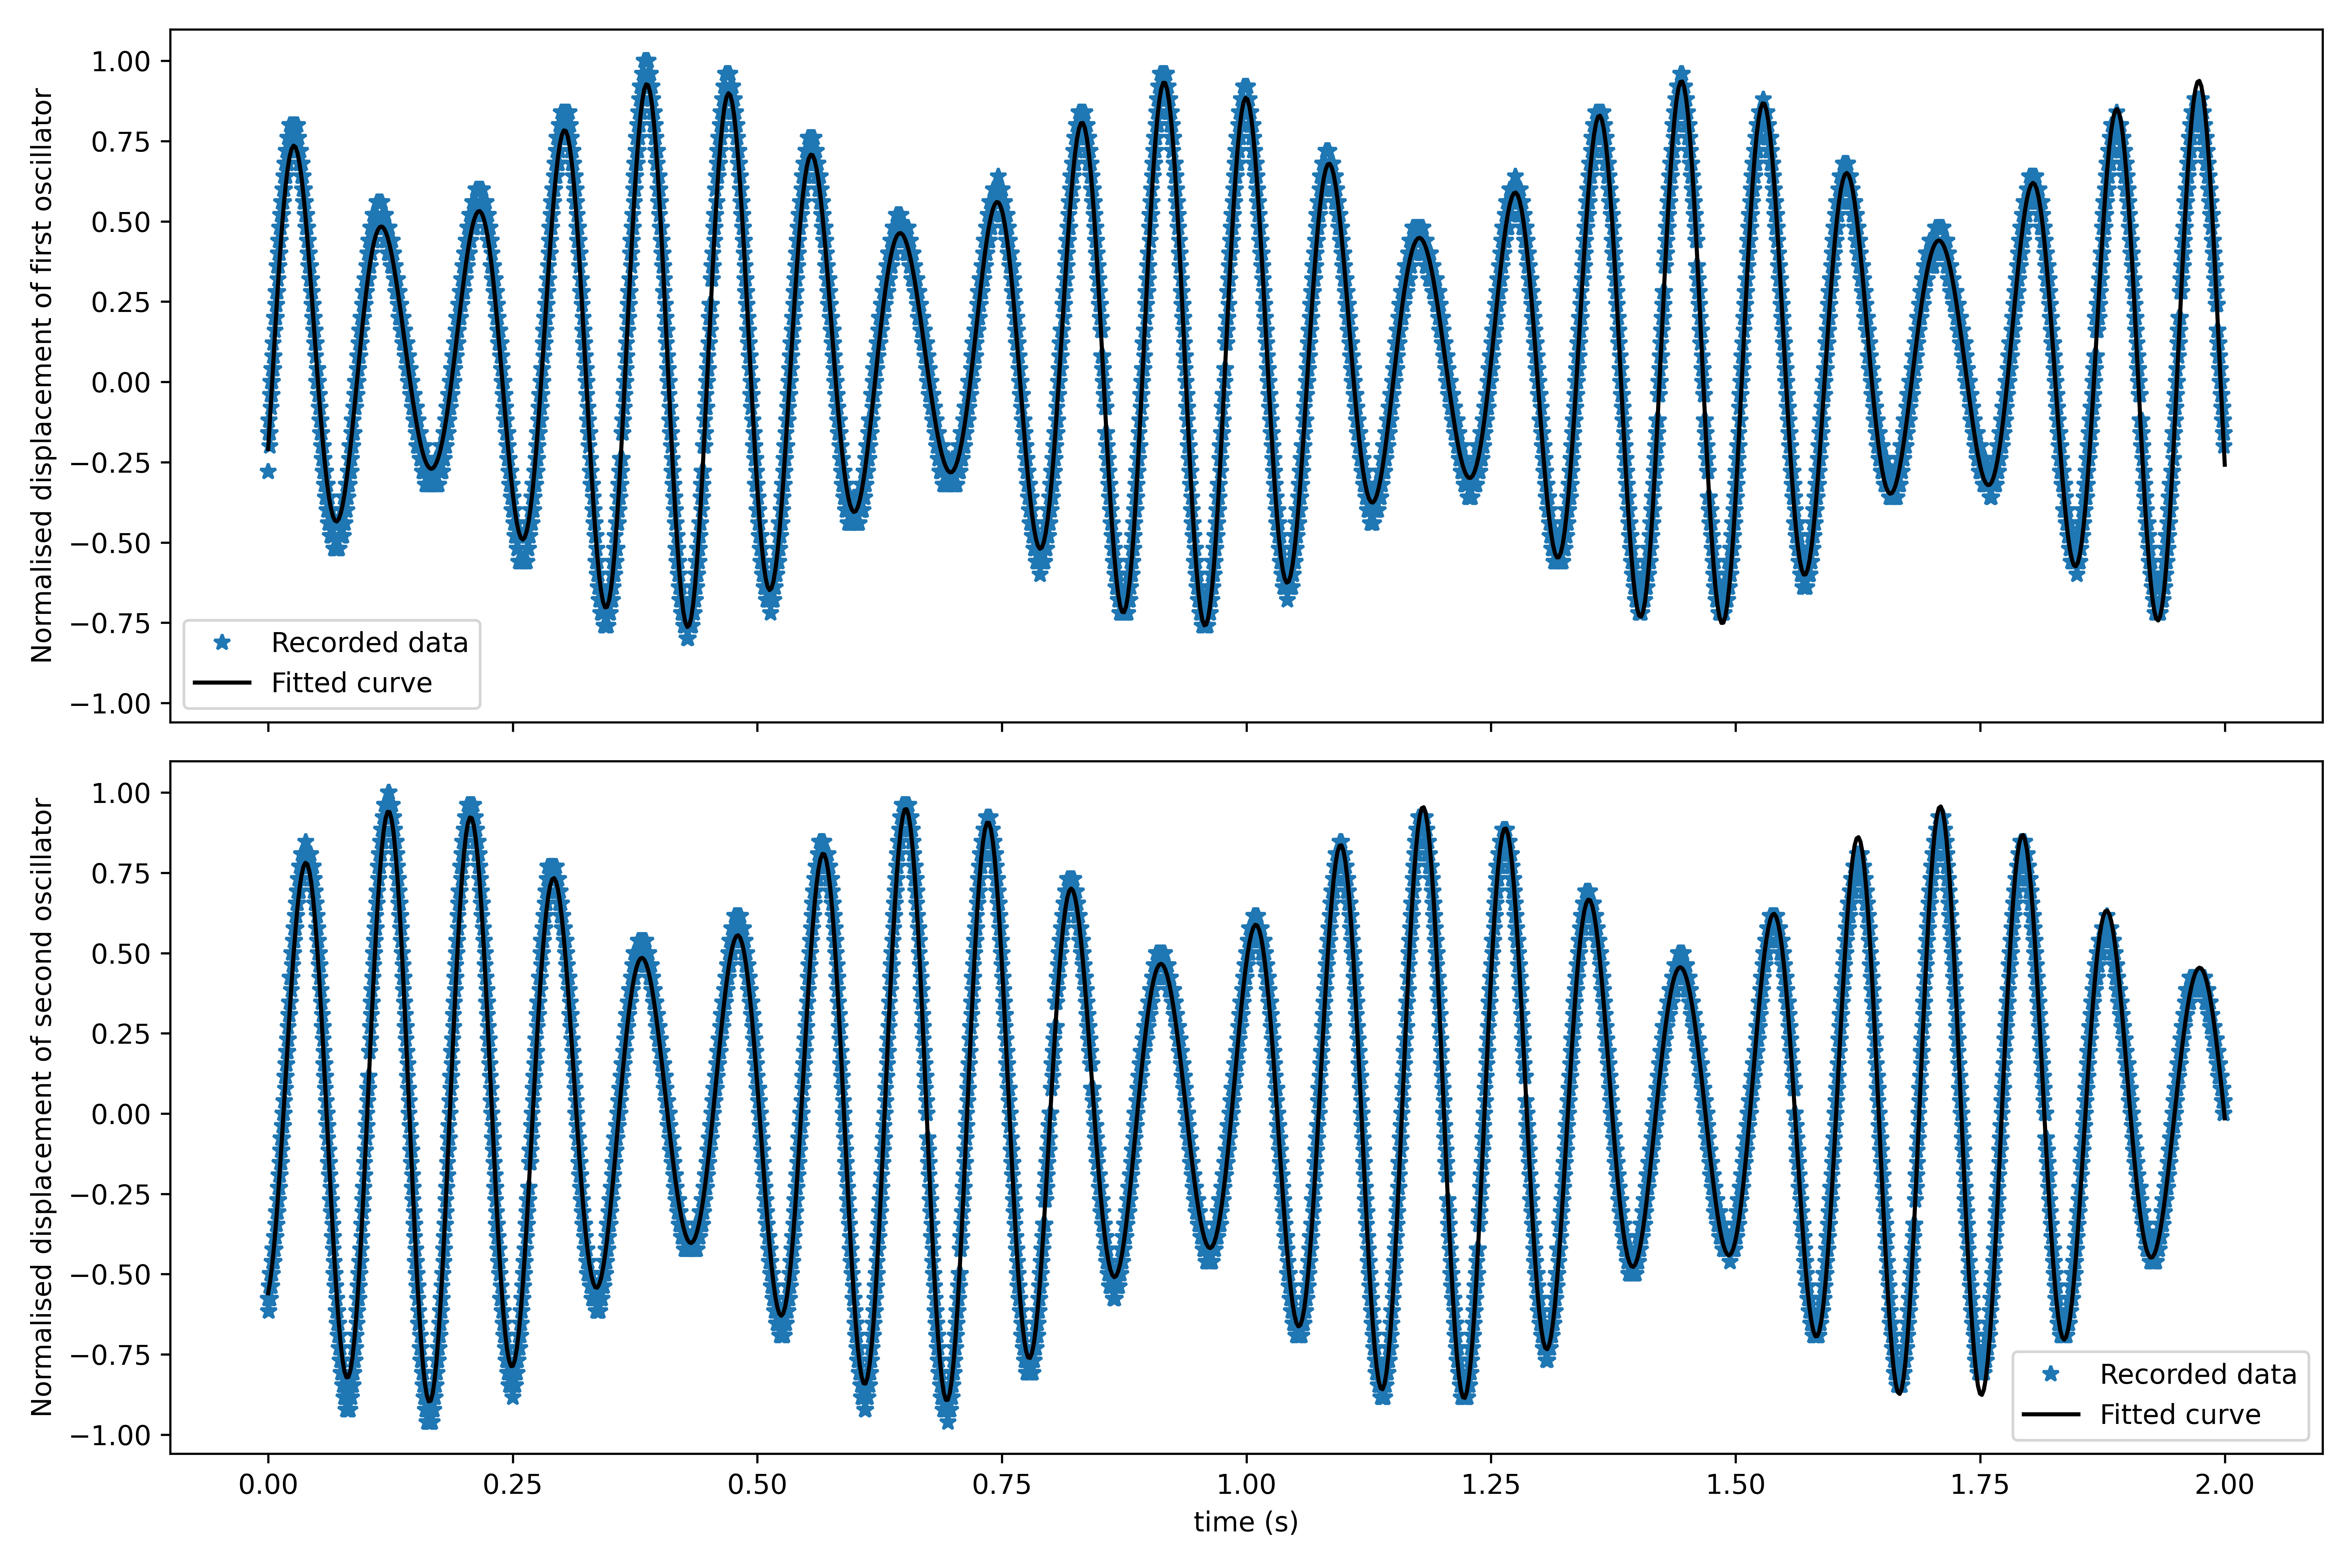
\includegraphics[scale=0.4]{01.png}
	\caption{Normalised displacements of the two oscillators as functions of time $ t $. The
		open circles are the experimental data, and the solid lines denote the fitted functions.}
	\label{fig:first}
\end{figure}

\begin{figure}[H]
	\centering
	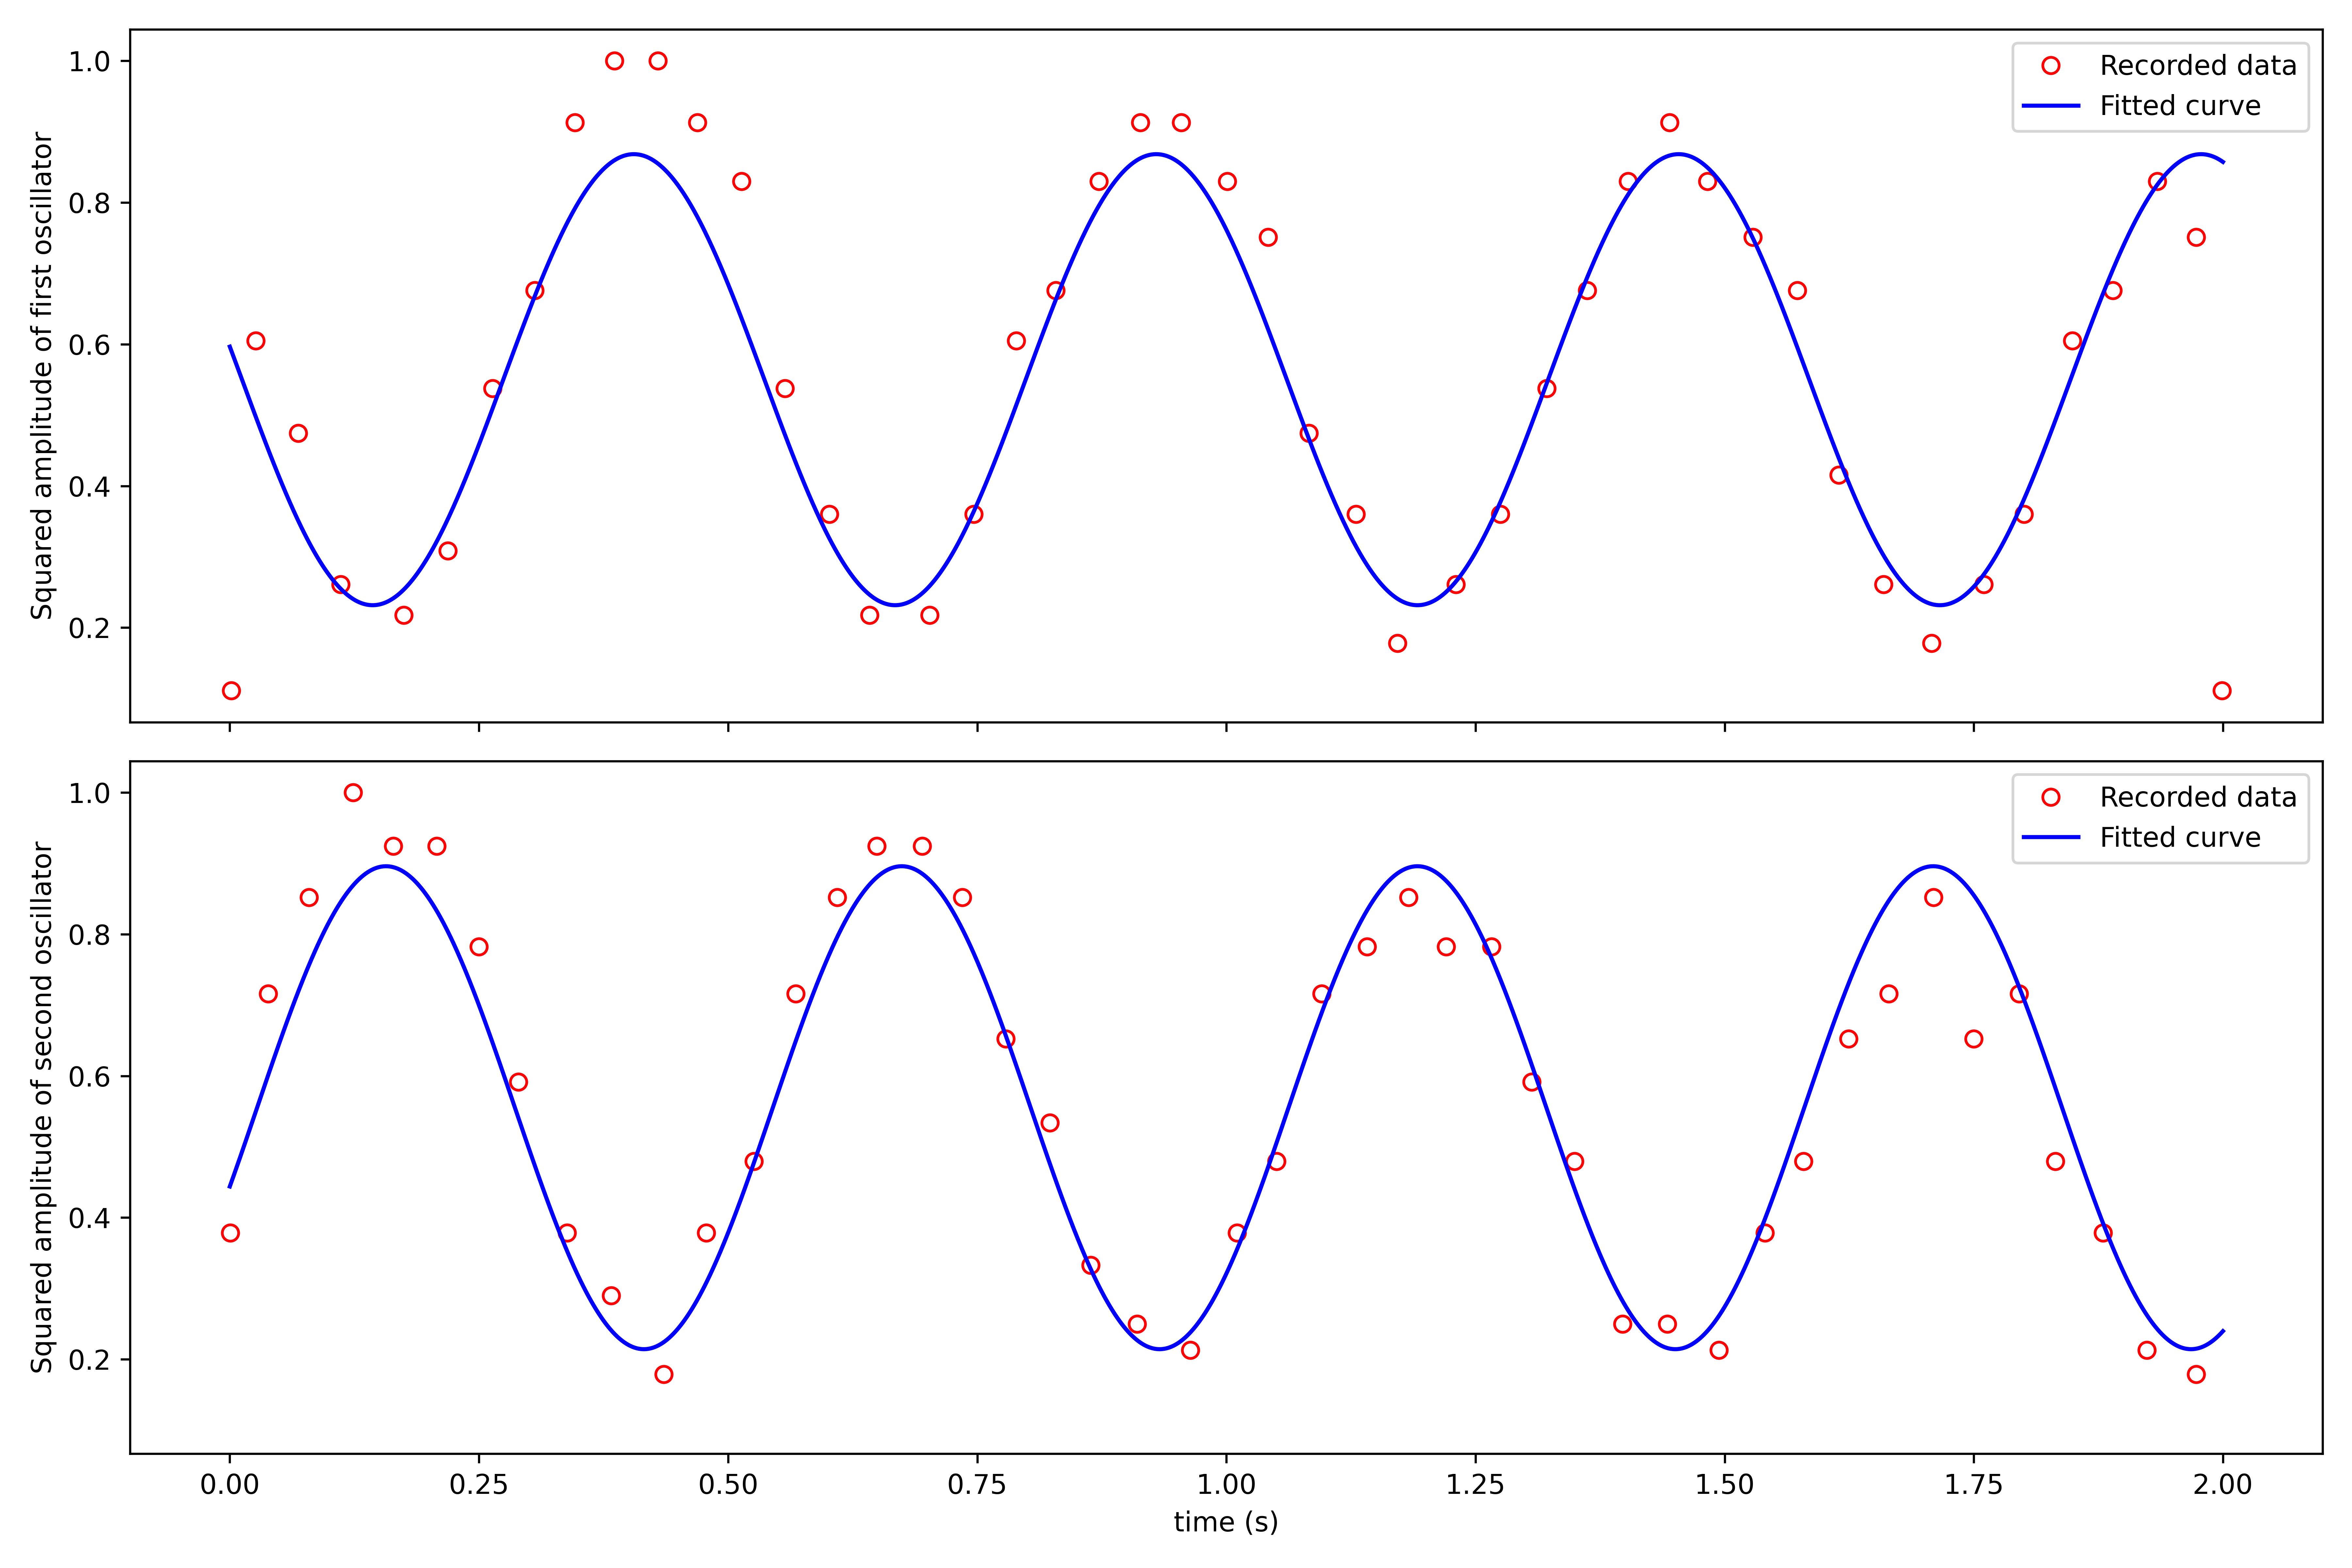
\includegraphics[scale=0.4]{01_squared.png}
	\caption{Squares of the fitted normalised amplitudes of the oscillators as functions of
		time. The open circles are the squares of the experimental amplitudes (obtained as the
		local extrema of the displacements), and the solid lines are the fitted functions}
	\label{fig:first_sq}
\end{figure}

Similarly the other plots were obtained and that gave us the fitting parameters. In total we used 19 data files, each of which gave the Rabi model parameters we needed to study the dependence of geometric phase with detuning. 

\section{Calculation of Rabi model parameters and the Geometric Phase}
Here we present the plots where we calculated the Rabi model parameters and the geometric phase and fitted thier functions.

\begin{figure}[H]
	\centering
	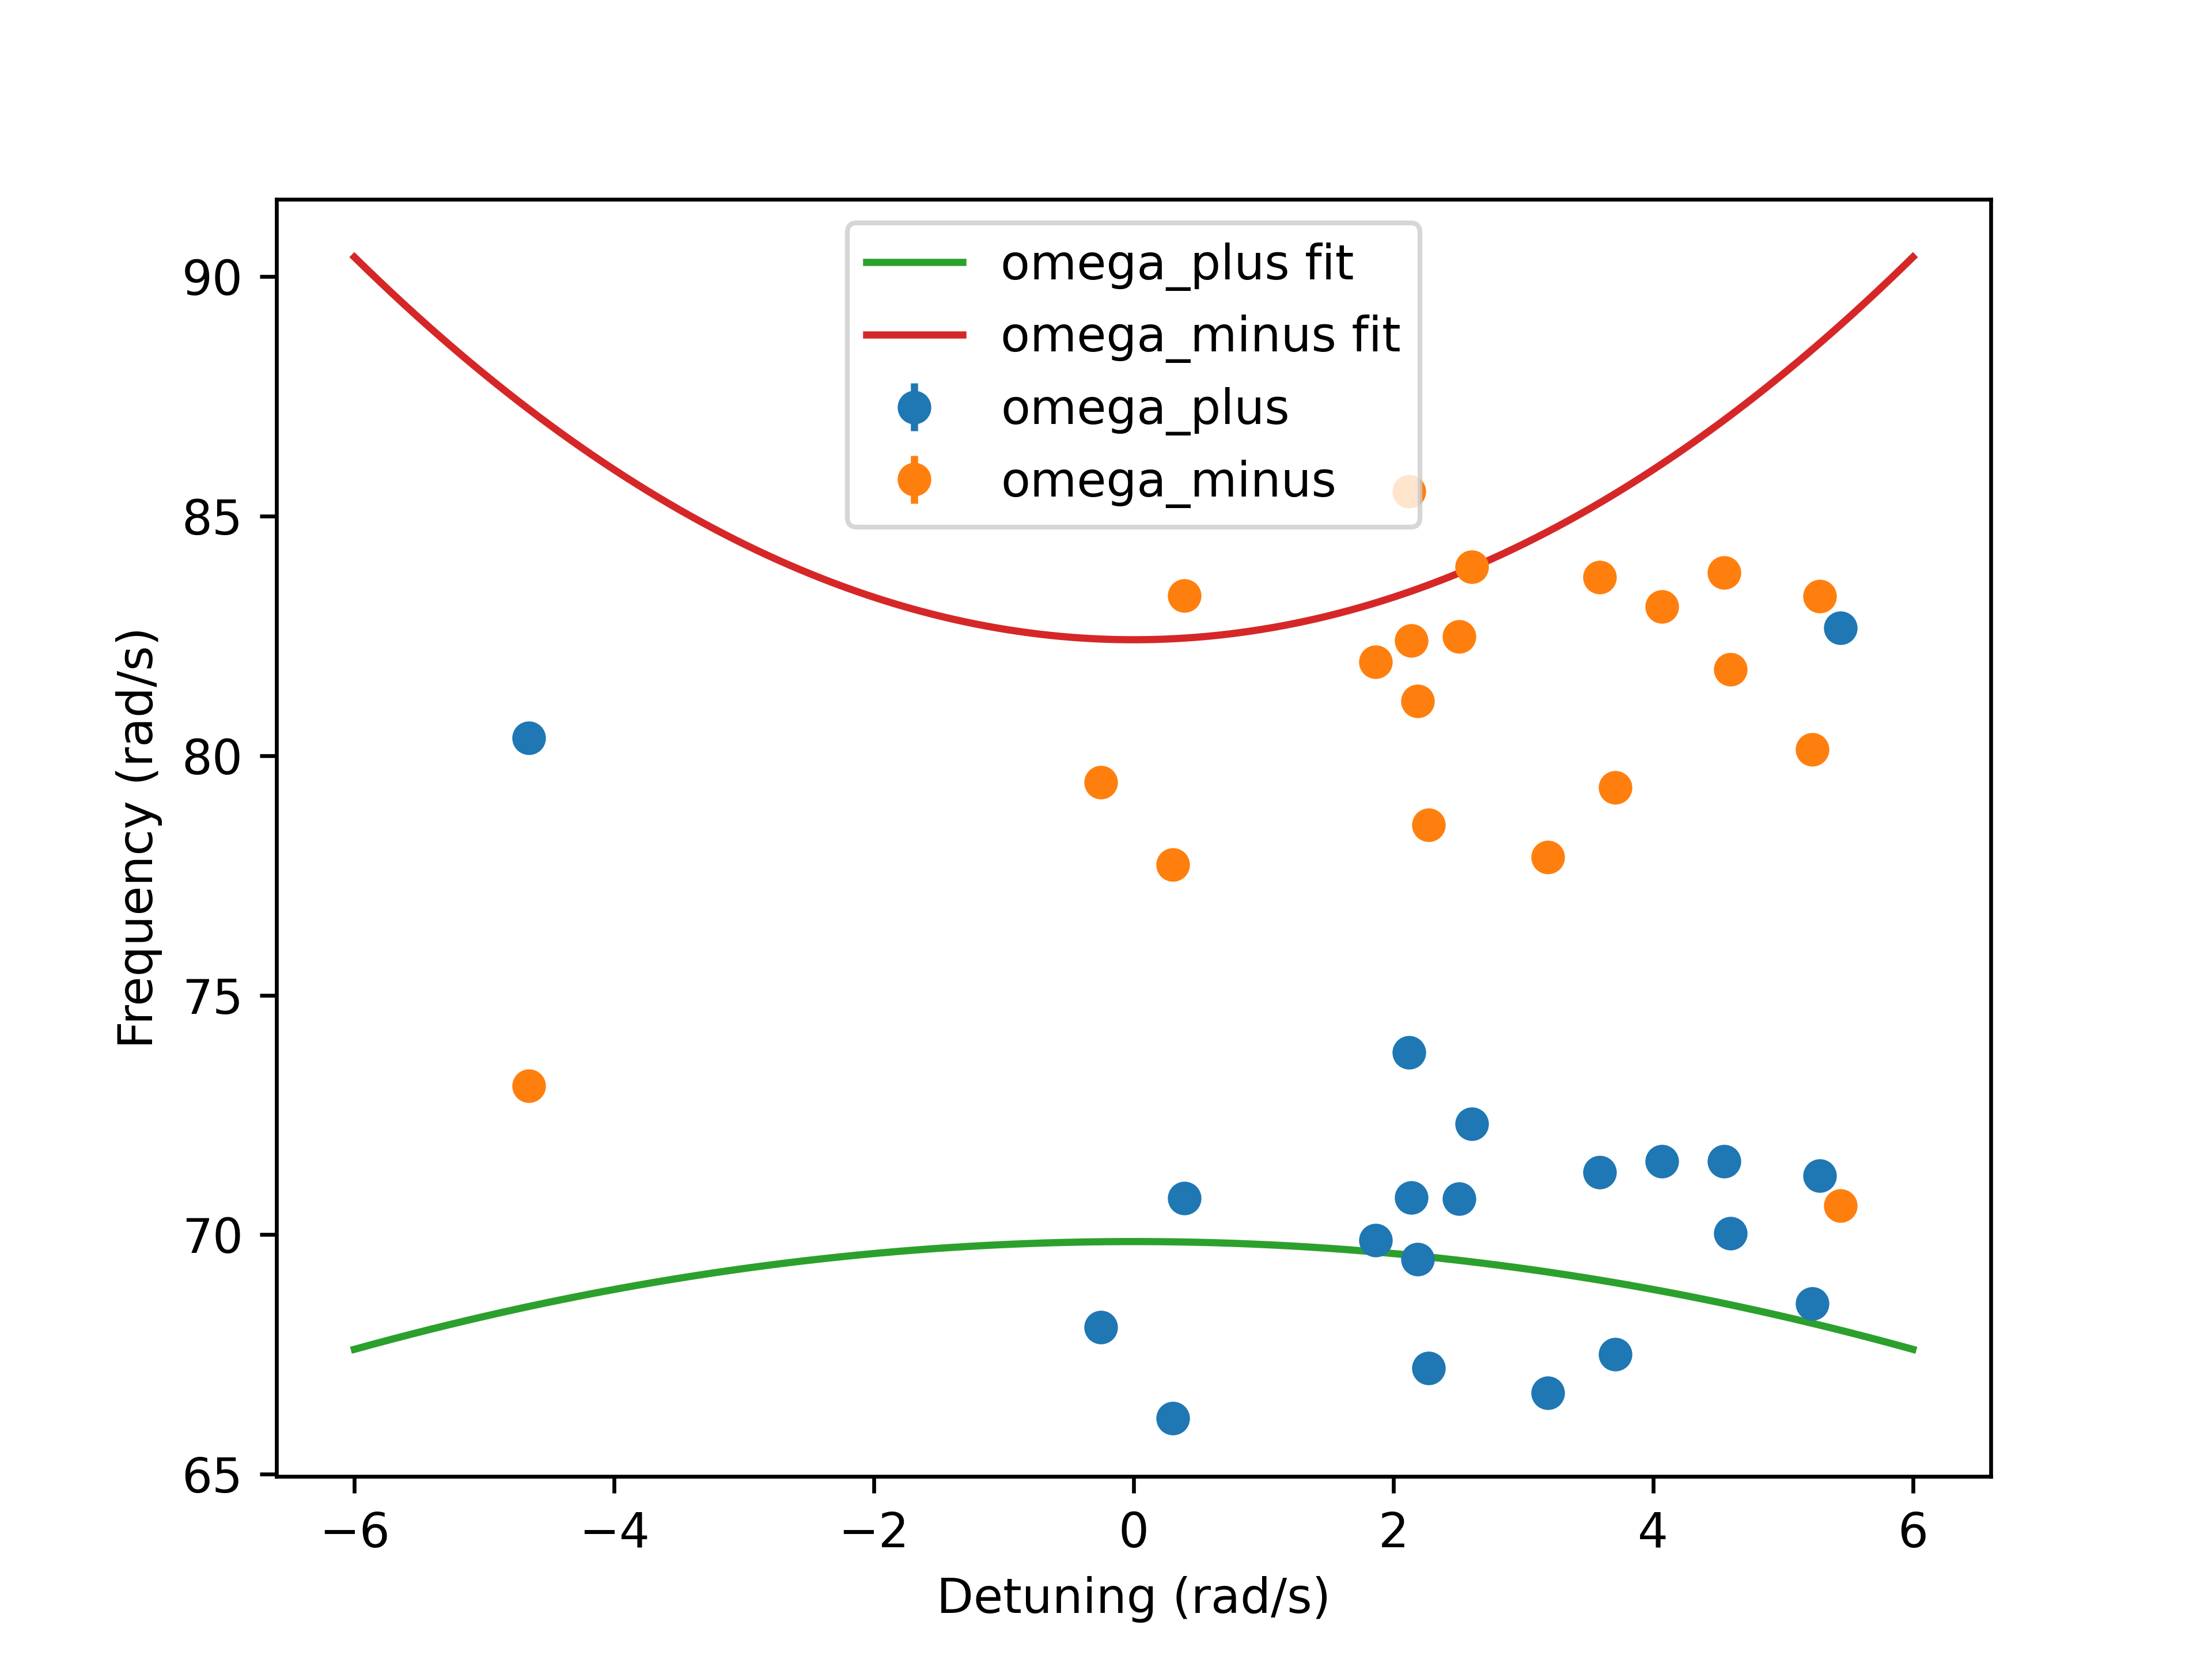
\includegraphics[scale=0.4]{20_freq_det.png}
	\caption{ Normal mode frequencies ($ \omega_{\pm} $) as functions of the detuning $ \Delta $. The circles are
		the experimental data, and the solid lines denote the fitted curves}
	\label{fig:first_sq}
\end{figure}

\begin{figure}[H]
	\centering
	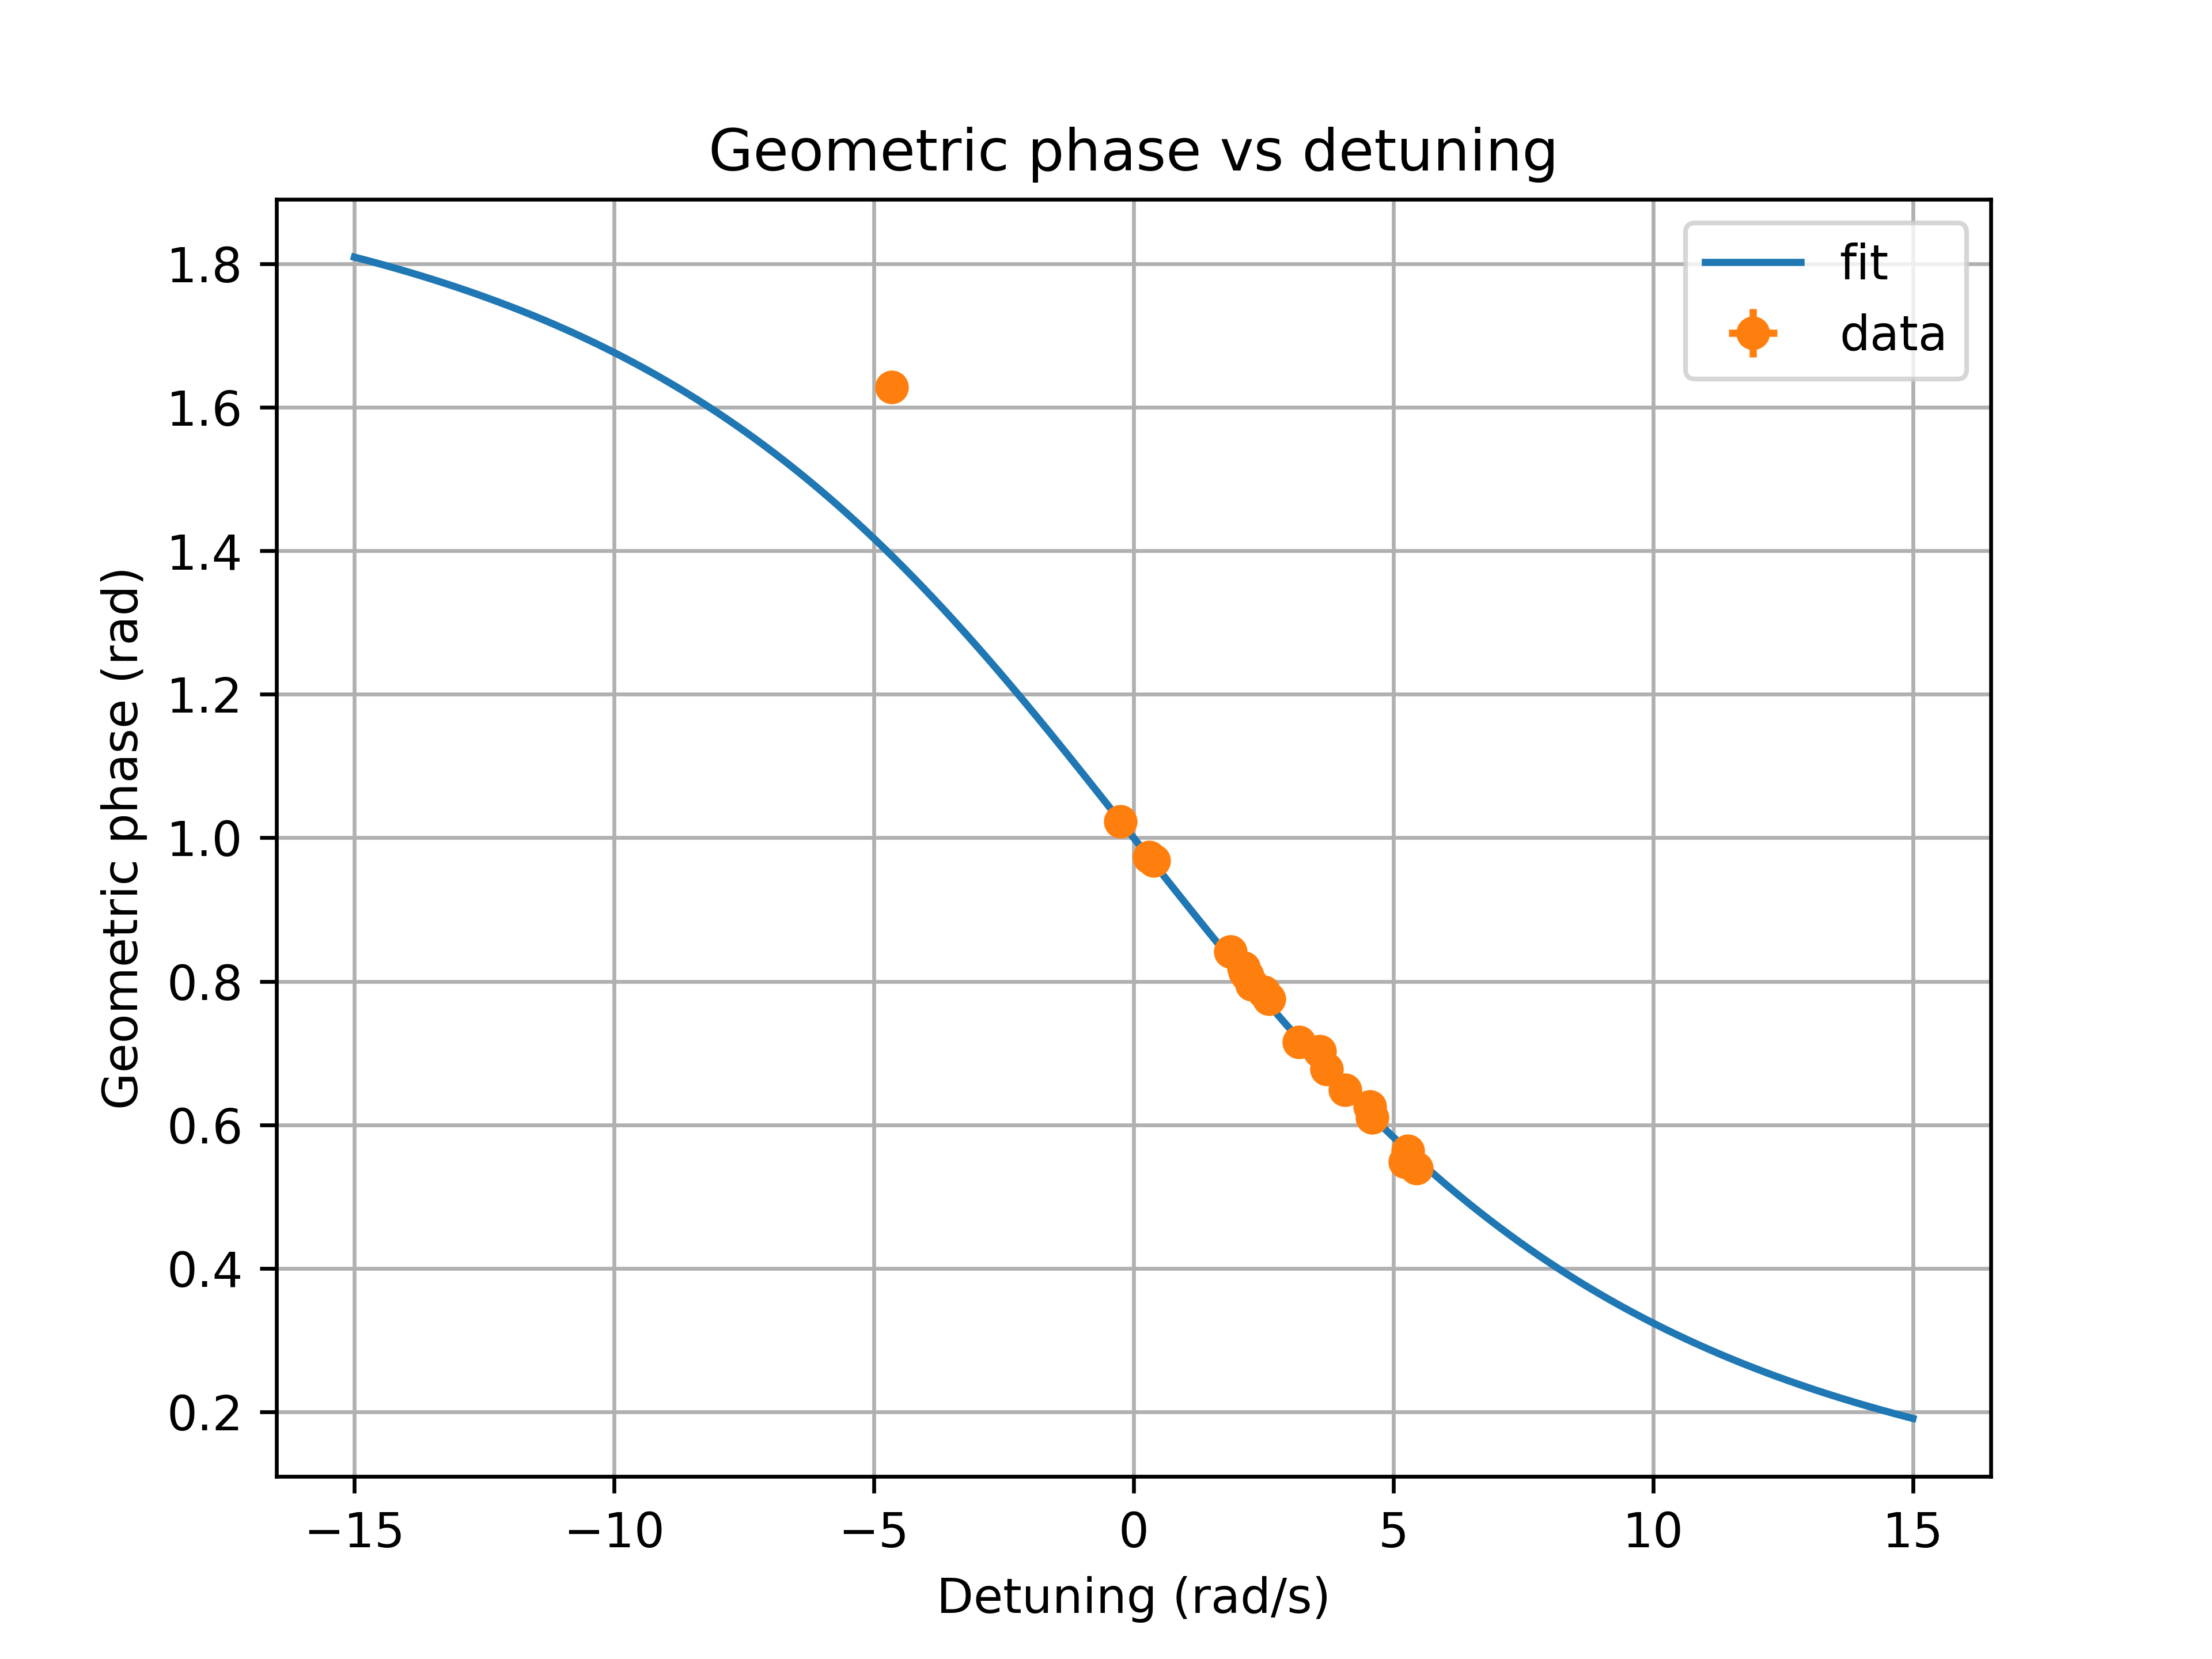
\includegraphics[scale=0.4]{Geometric_phase.png}
	\caption{Geometric phase $ \phi_{G} $ as a function of the detuning $ \Delta $. The circles are the
		experimental data, and the solid line denotes the fitted curve. }
	\label{fig:first_sq}
\end{figure}

\begin{figure}[H]
	\centering
	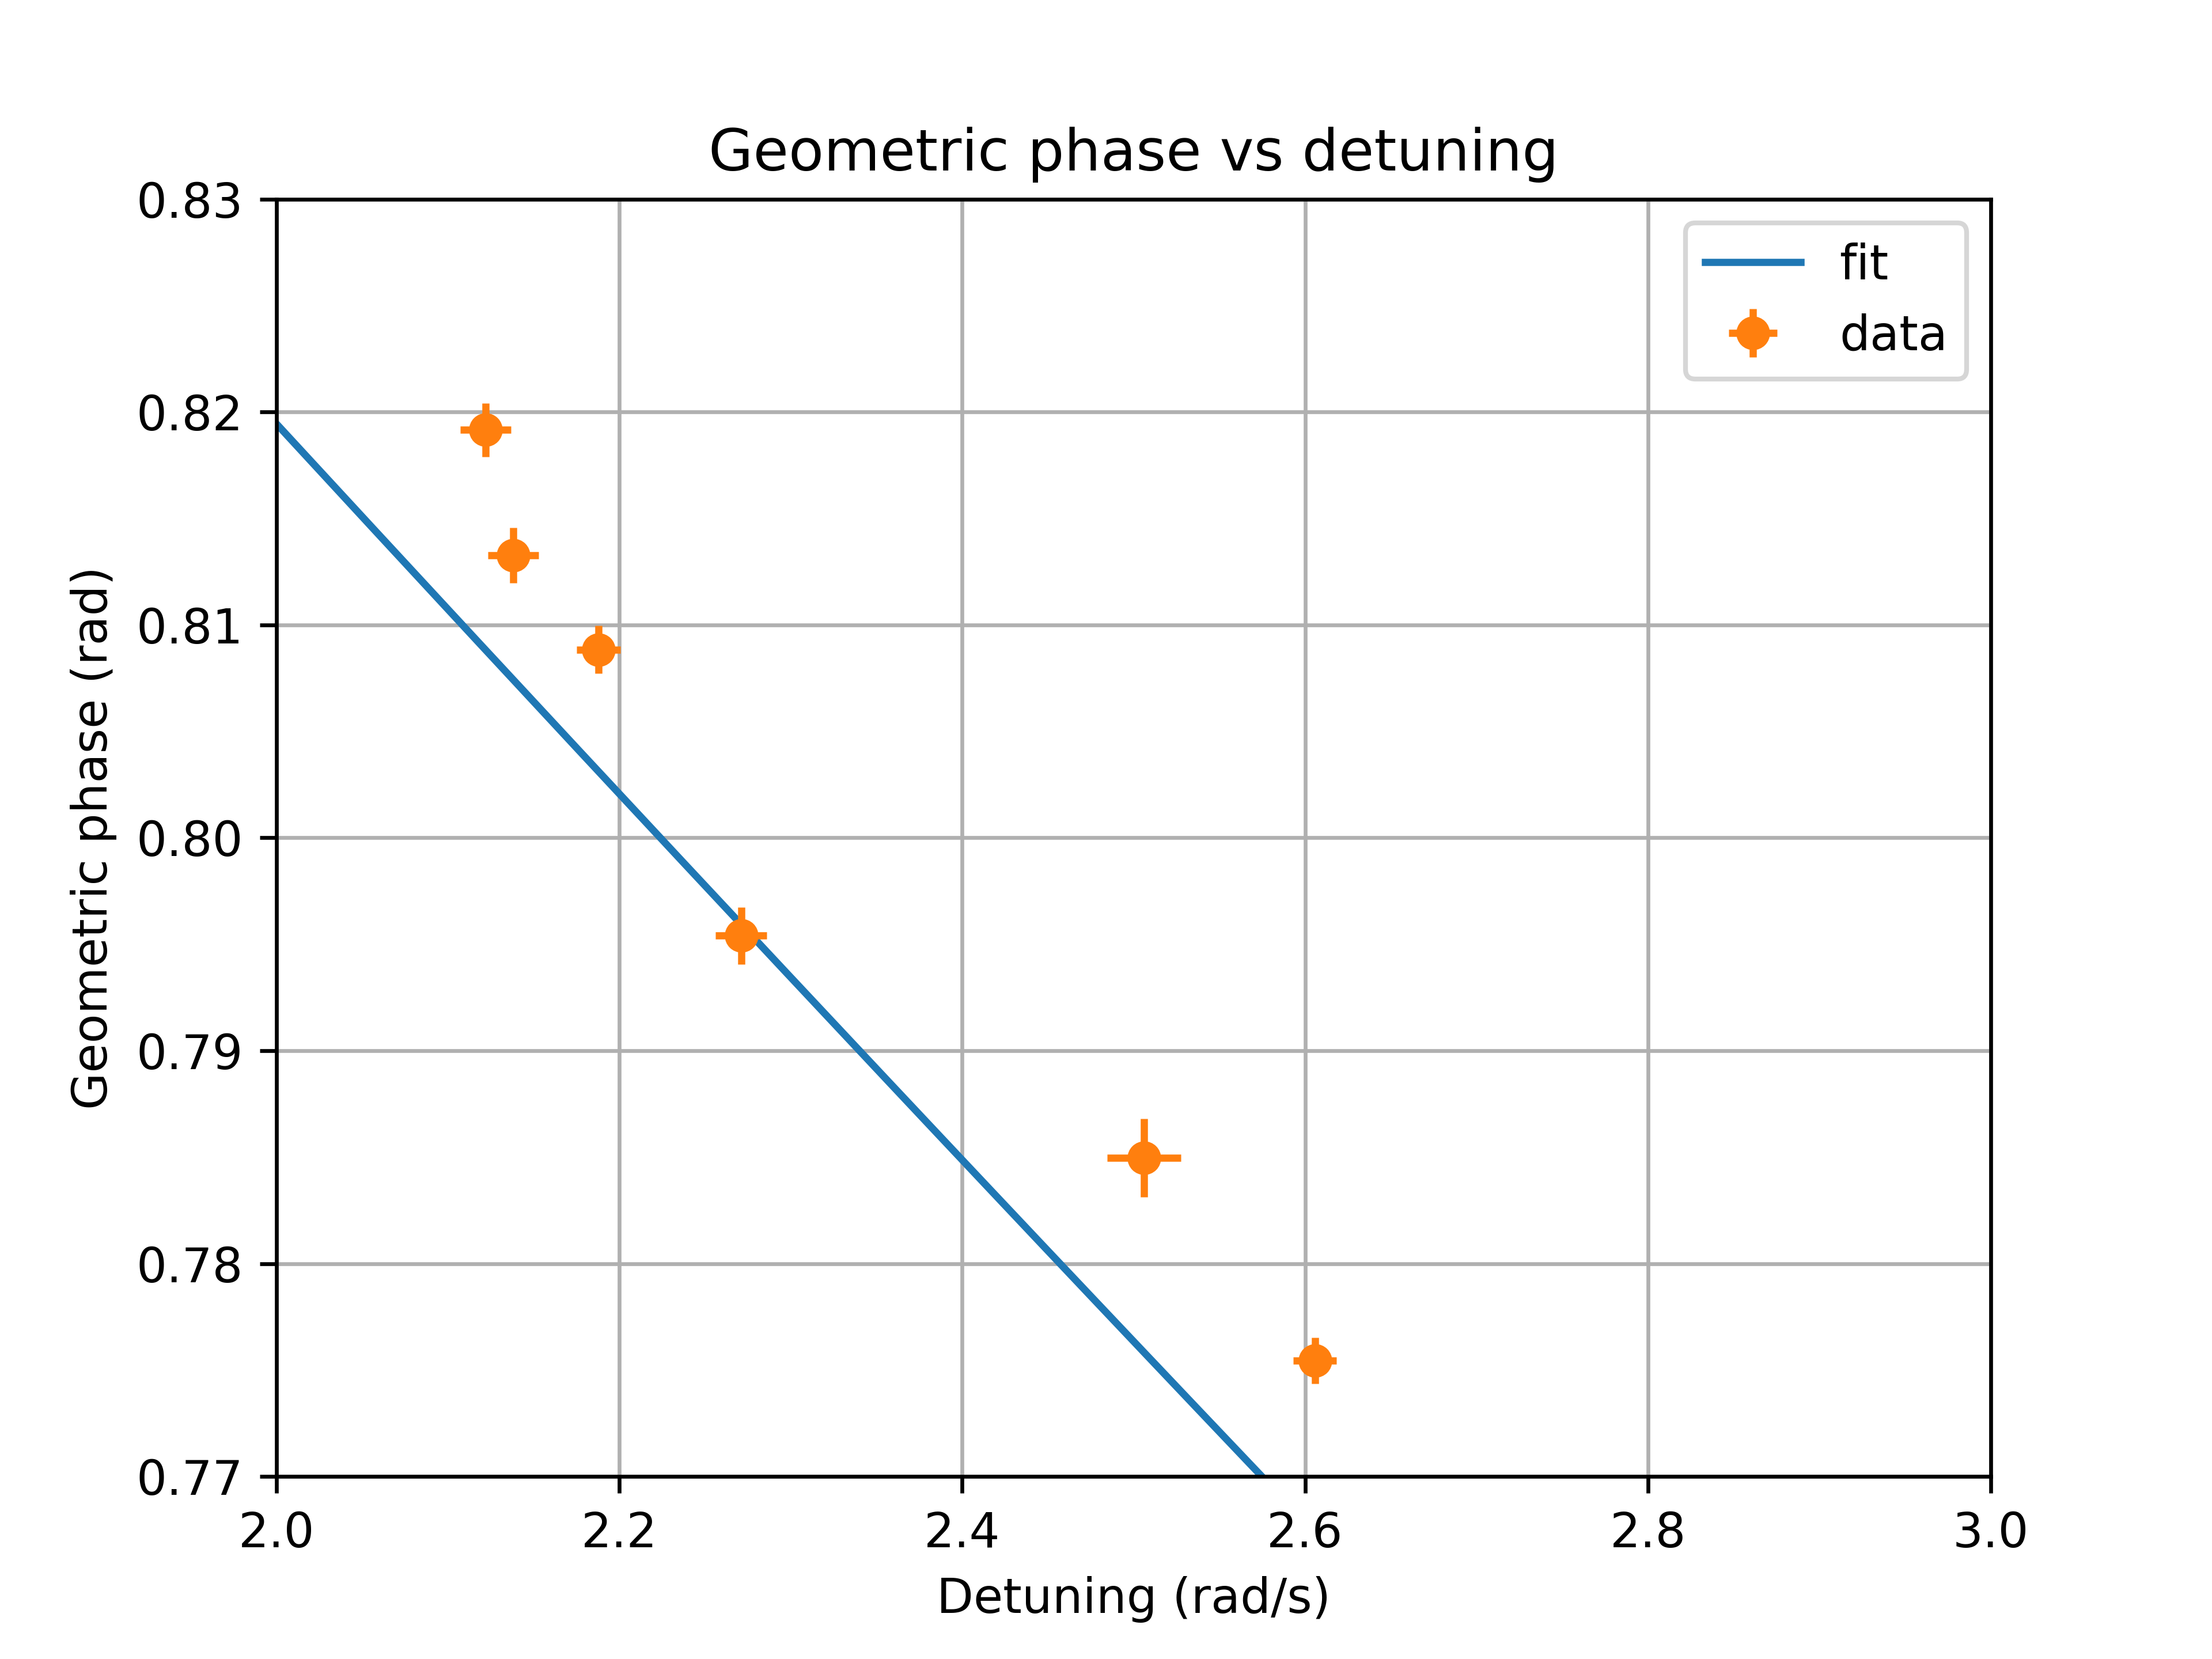
\includegraphics[scale=0.4]{Zoomed_in_geometric_phase.png}
	\caption{Zoomed in version of the geometric phase plot to show the error bars}
	\label{fig:first_sq}
\end{figure}
\setcounter{equation}{0}
\setcounter{table}{0}
\setcounter{figure}{0}
%\baselineskip 24pt
